\documentclass{article}

\usepackage[english]{babel}
\setlength\parindent{0pt} % Removes all indentation from paragraphs
%\usepackage{times} % Uncomment to use the Times New Roman font

\usepackage{color}
	\definecolor{darkred}{rgb}{0.55, 0.0, 0.0}
	\definecolor{keywords}{RGB}{255,0,90}
	\definecolor{comments}{RGB}{0,0,113}
	\definecolor{red}{RGB}{160,0,0}
	\definecolor{green}{RGB}{0,150,0}

\usepackage{amssymb,amsmath}
\usepackage{mathtools}

\usepackage{placeins}

\usepackage{wrapfig}
\usepackage{graphicx}
\usepackage{caption}
\usepackage{subcaption}

\usepackage{hyperref}

\usepackage{listings}
\lstset{language=Python, 
        basicstyle=\ttfamily\small, 
        keywordstyle=\color{keywords},
        commentstyle=\color{comments},
        stringstyle=\color{red},
        showstringspaces=false,
        identifierstyle=\color{green},
        title=\lstname}
%------------------------------------------------------------------------------%
%------------------------------------------------------------------------------%                                   
\title{Machine Learning \\ \bf{Exercise 4: Generative non-parametric classification:\\
								Naive Bayes and Density trees} } % Title
%------------------------------------------------------------------------------%                                   
% Document
%------------------------------------------------------------------------------%                                   

\begin{document}

\maketitle

\begin{center}
\begin{tabular}{l l}
Group: &  Sergej Kraft \\
       & Elias Roeger \\
       & Ekaterina Tikhoncheva \\ 
\end{tabular}
\end{center}

\tableofcontents

\section{Data set}

In this exercise we used the MNIST dataset, containing images of the handwritten digits. The size of the original images was to big for our purpose, so we used provided compressed version of the dataset, from which we picked up images with handwritten threes and eights.

For further dimension reduction of the feature space to the size of $2$ we used as corresponding function, we wrote for the exercise $2$: 

\lstinputlisting[language=Python]{dr.py}

\FloatBarrier

\section{Naive Bayes}

\subsection{Classification}

As we know from the theory the assumption of the naive Bayes Methode is, that all features are independent. That means:
$$p(y=k|x)=\frac{\prod_{j=1}^d p(x_j|y=k) p(y=k)}{\prod_{j=1}^d p(x_j)}$$

Our aim is therefore to learn for each class $k$ one dimension histograms $p(x_j|y=k)$ and prior $p(y=k)$.

The prior $p(y=k)$ is simply $N_k/N$, where $N_k$ is the number of elements in the training set from the class $k$ and $N$ is the size of the whole training set.
To learn the histograms we need an appropriate binning. We selected a common bin number for each dimension in the following way: for each dimension we used the Freeman-Dice rule to compute the bin width. From the bin width we got the necessary number of bins pro dimension and class. We selected the smallest necessary number of bin over all dimensions and recalculated the corresponding bin width.

\begin{lstlisting}[language=Python]
# 			Choose proper bin size
def chooseBinSize(trainingx):
  
    n = trainingx.shape[0]
    d = trainingx.shape[1]
    
    # Choose bin width 
    dx = np.zeros(d, dtype = np.float128)
    m = np.zeros(d, dtype = np.int32)
    for j in range(0,d):
	# for each dimension apply Freeman-Diace Rule
        ind_sort =  np.argsort(trainingx[:,j]); # j-th feature dimension
        IQR = trainingx[ind_sort[3*n/4],j] - trainingx[ind_sort[n/4],j]        
        dx[j] = 2*IQR/np.power(n, 1/3.)        
        if dx[j]<0.01:
           dx[j] =  3.5/np.power(n, 1/3.)        
        m_j = (np.max(trainingx[:,j])-np.min(trainingx[:,j]))/dx[j]   
        m[j] = np.floor(m_j) + 1       
    # end for j
        
    L = np.min(m);  # total number of bins as minimum over all bin sizes
		    # in all dimensions
    
    # recalculate bin width according to the new bin size L
    for j in range(0,d):
        dx[j] = (np.max(trainingx[:,j])-np.min(trainingx[:,j]))/float(L-1)
    # end for j 
    
    return L, dx
# end chooseBinSize
\end{lstlisting}

The learning function uses the given number of bins and bin width to calculate $1$-dimensional histograms pro class and dimension:

\begin{lstlisting}[language=Python]
##                          Naive Bayes Training
# determine priors  and likelihoods (for each feature and class individual 
# histogram <=> 4 histogramms   ) 
def naiveBayes_train_single_class(trainingx, trainingy, c, dx, L):
    # we consider one class c
    #    
    # trainingx is our training set    
    # trainingy are class labels for each element from trainingx
    # dx bin width
    # L total number of bins pro dimension
    
    n = trainingx.shape[0]      # size of the training set
    d = trainingx.shape[1]      # size of the feature space
    
    # find  in training set all members of the class c
    xc = trainingx[trainingy==c, :]        # Class of digit c
    nc = xc.shape[0]

    ## Priors
    prior = nc/float(n)
    
    ## Likelihood p(x|y=c)
    
    likelihood = np.zeros((d, L), dtype = np.float32)
  
    for j in range(0,d):
        for i in range(0,nc):    
            l = np.floor(xc[i,j]/dx[j])+1 # bin 
            if l>=L+1:
                print xc[i,j]
            likelihood[j, l-1] = likelihood[j, l-1] + 1
        # end for i=1..nc
        likelihood[j,:] = likelihood[j,:]/float(nc)    
    #end for j=1..d                 
    
    return prior, likelihood
#end def naiveBayes_train
\end{lstlisting}

If we visualize calculated histograms we get following result:

\begin{figure}[hb]
        \centering
        \begin{subfigure}[b]{0.5\textwidth}
                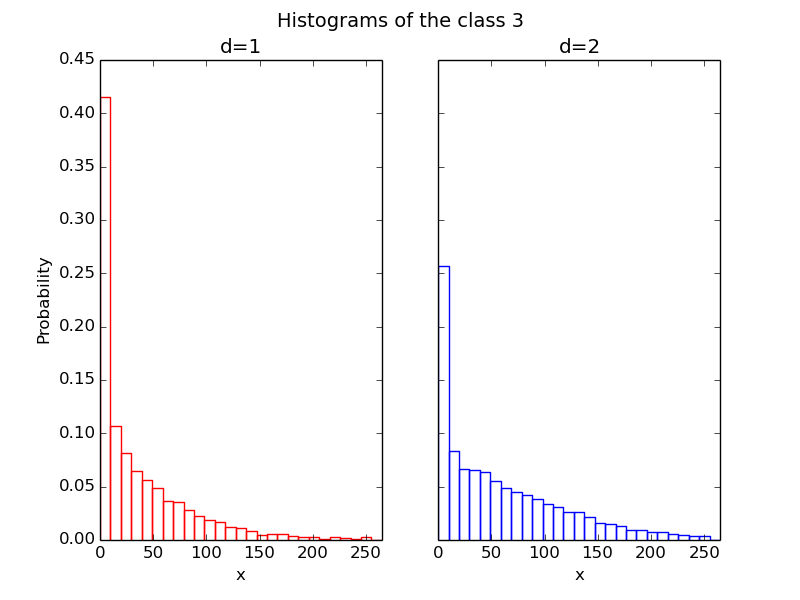
\includegraphics[width=\textwidth]{../histograms3.png}
                \caption{Class of handwritten threes}
        \end{subfigure}%
        \begin{subfigure}[b]{0.5\textwidth}
                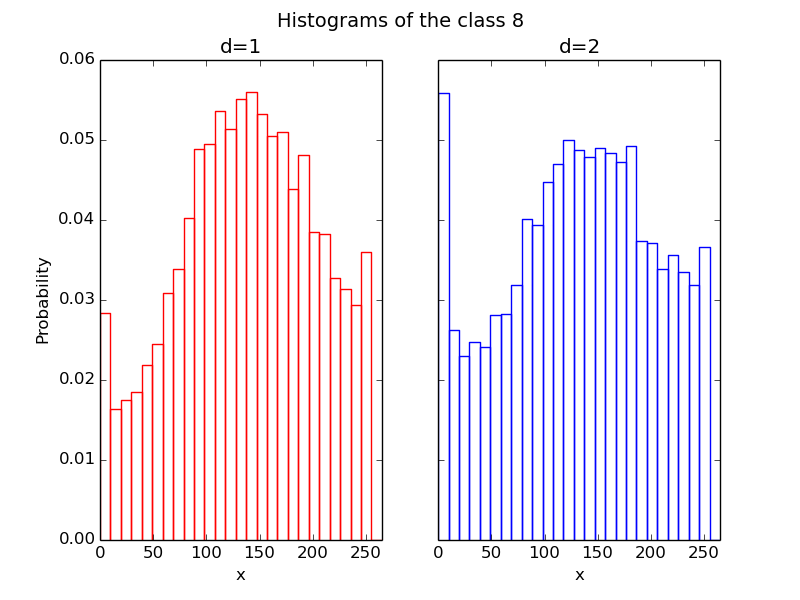
\includegraphics[width=\textwidth]{../histograms8.png}
                \caption{Class of handwritten eights}
        \end{subfigure}
        \caption{1 dimensional histograms pro class and dimension}
        \label{img4}
\end{figure}

One the next two images we can see the visualization of the likelihoods for each class:

\begin{figure}[ht]
        \centering
        \begin{subfigure}[b]{0.5\textwidth}
                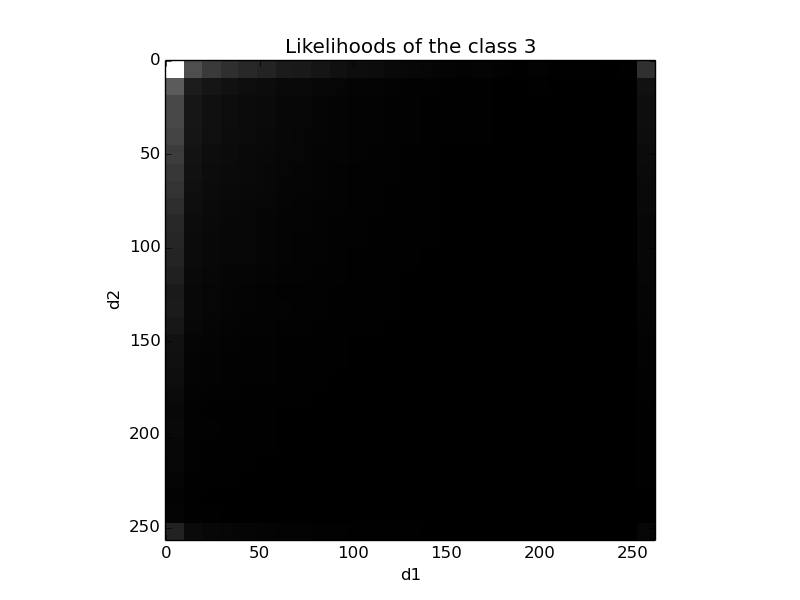
\includegraphics[width=\textwidth]{../likelihoods3.png}
                \caption{Class of handwritten threes}
        \end{subfigure}%
        \begin{subfigure}[b]{0.5\textwidth}
                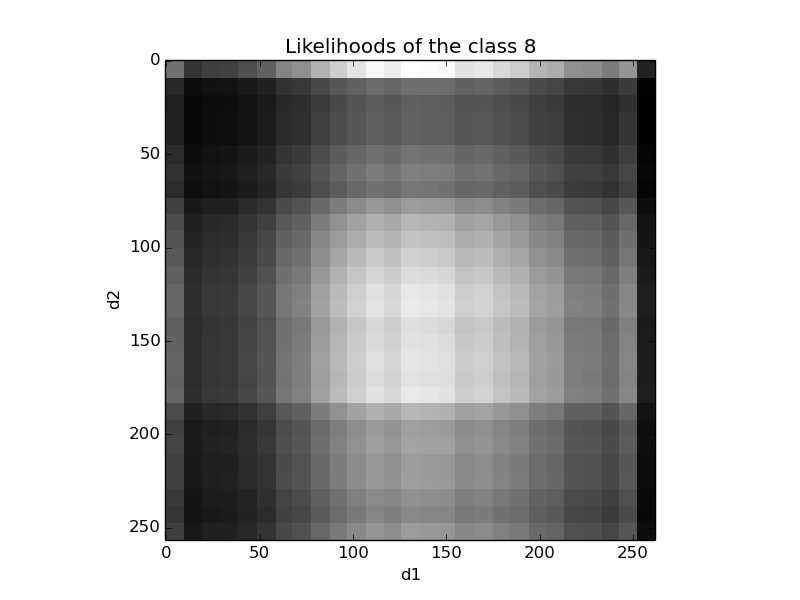
\includegraphics[width=\textwidth]{../likelihoods8.png}
                \caption{Class of handwritten eights}
        \end{subfigure}
        \caption{2D likelihoods}
        \label{img4}
\end{figure}

\FloatBarrier

After learning phase of the classifier we apply it on the test set images. The correct classification rate of the classifier is $0.8266$ (error rate = $0.1734$).

The classification function: 
\begin{lstlisting}[language=Python]
##                          Naive Bayes Classifier
#
def naiveBayesClassifier(testx, p3, p8, p_k3, p_k8, dx):
    n = testx.shape[0]
    
    prediction = np.zeros(n, dtype = np.int8)
        
    for i in range(0,n):
        x = testx[i,:]
        
        # p(y = 3| x)
        
        l_y3_d1 = np.floor(x[0]/dx[0])+1 # bin number
        p_x_y3_d1 = p_k3[0,l_y3_d1-1]

        l_y3_d2 = np.floor(x[1]/dx[1])+1 # bin number
        p_x_y3_d2 = p_k3[1,l_y3_d2-1]
        
        p_y3_x = p_x_y3_d1*p_x_y3_d2*p3
        
        # p(y = 8| x)

        l_y8_d1 = np.floor(x[0]/dx[0])+1 # bin number
        p_x_y8_d1 = p_k8[0,l_y8_d1-1]

        l_y8_d2 = np.floor(x[1]/dx[1])+1 # bin number
        p_x_y8_d2 = p_k8[1,l_y8_d2-1]
        
        p_y8_x = p_x_y8_d1*p_x_y8_d2*p8
        
        # argmax (p_y3_x, p_y8_x) 
        #print p_y3_x
        if p_y3_x>p_y8_x :
            prediction[i] = 3
        else:
            prediction[i] = 8
        # end if        
        
    # end for i
    return prediction
#end def naiveBayesClassifier
\end{lstlisting}

\subsection{Generate threes}
To construct a new digits we applied our learning algorithm to the full dimension training set ($81$ dimension) to get the likelihood for the class of threes. The sampling algorithm we used is : 
	\begin{itemize}
	\item Since we assumed, that all features are independent, we can sample in each dimension separately
	\item So for each dimension calculate the cumulative distribution function (CDF); pick the uniform distributed number 	in $\alpha\in[0,1)$; calculate for each $CDF_j, j=1\dots d$, $\alpha$-quantil; return the rounded value of the $\alpha$-quantil as the $j{th}$ component of the new number.
	\end{itemize}	

Here are some results of the described generation function and the code of the function:

\begin{figure}[ht]
        \centering
        \begin{subfigure}[b]{0.5\textwidth}
                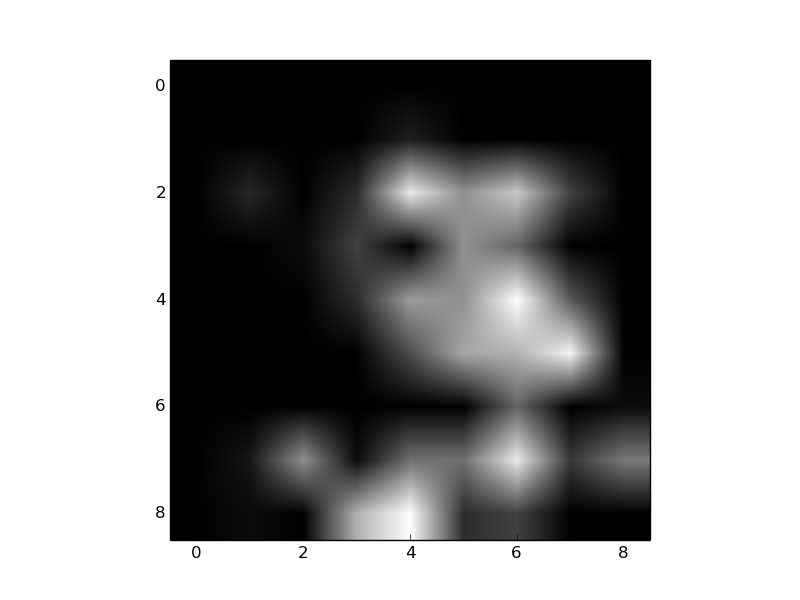
\includegraphics[width=\textwidth]{../new3nB_1.png}
        \end{subfigure}%
        \begin{subfigure}[b]{0.5\textwidth}
                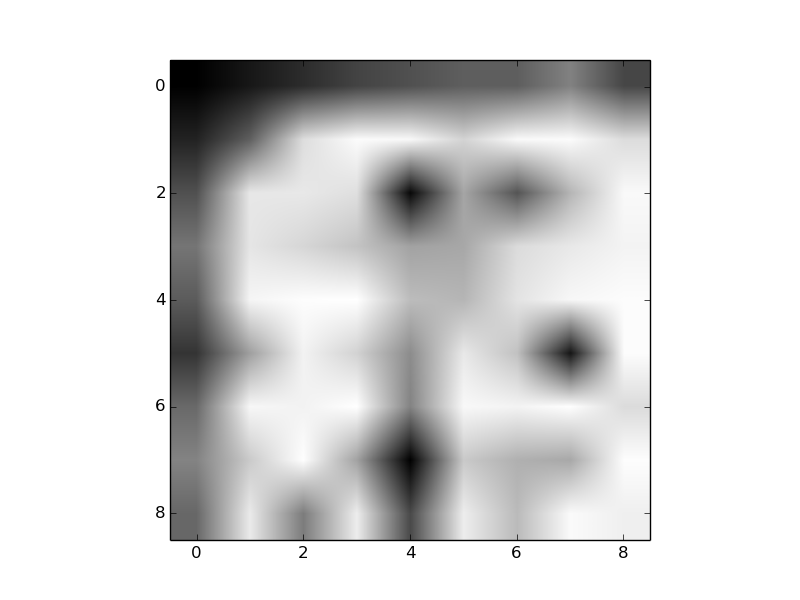
\includegraphics[width=\textwidth]{../new3nB_2.png}
        \end{subfigure}
        \begin{subfigure}[b]{0.5\textwidth}
                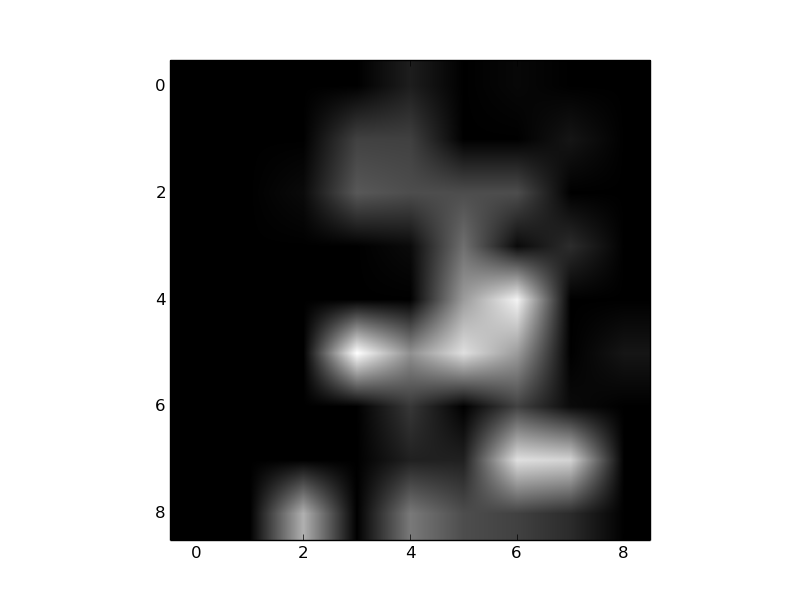
\includegraphics[width=\textwidth]{../new3nB_3.png}
        \end{subfigure}        
        \caption{Generated threes}
\end{figure}

\FloatBarrier

\begin{lstlisting}[language=Python]
# Generate Number from the given pdf
# samply in each of d dimensions independently
def generate_number(pdf,dx):
    
    d = pdf.shape[0]    # number of dimension
    
    newnumber = np.zeros(d, dtype = np.int32)
    # calculate cumulative distribution function (cdf) from pdf
    cdf = np.zeros(pdf.shape, dtype = np.float32)
    for j in range(0, d):
        cdf[j,:] = np.cumsum(pdf[j,:])
    # end for
        
    for j in range(0,d):
        # randomly select a uniformly distribut number in range [0., 1.)
        alpha = random.random()
        # calculate quantile on the level alpha
        dist = abs(cdf[j,:] - alpha)
        binx = np.argsort(dist)
        
        newnumber[j] = np.floor(dx[j]*binx[0])+1
    # for j    
    return newnumber
# def generate_number(pdf)
\end{lstlisting}

The whole code to the naive Bayes part can be found in the file $naiveBayes.py$.

\section{Density trees}

As opposite to the naive Bayes method density tree method should keep the possible interactions between features.

\subsection{Building the DT}
We wrote recursive function $DT\_cut$, which split each node of the tree in two parts and call itself in each of two new nodes. The inputs arguments are the whole number of points in the training set, list of the leaves nodes, current node, depth of the current node and split method.

The first call is made from the function $DT\_learning(trainingx, trainingy, c, splitmethod)$ which creates the root node - node containing all points of the training set.

The result of the learning is returned in form of the list with leaves nodes.

We tried out different termination criteria, such as restriction of the allowed depth or minimum density/number of points in the leaf nodes, but were not satisfied with none of them. The restriction of the allowed depth was often not sufficient to obtain a good probability distribution. Condition on minimum density/number of points led sometimes to overflow of the stack in cases of few points in a big bin. So we chose a combination of the minimum density condition supported with the condition, that $N_{bin}/N$ is not already to small. The idea is, that if $N_{bin}/N$ is already too small, the probability $N_{bin}/NV_{bin}$ would be even smaller and that would lead at the end to the distribution with values around zero.

\begin{lstlisting}[language=Python]
#               Learning DT         
# we consider one class at time    

def DT_learning(trainingx, trainingy, c, splitmethod):
    # in this version wir use naive split criterion on the nodes of the DT
    print "Learning DT for the class {}". format(c)
    
    n = trainingx.shape[0]      # size of the training set
    d = trainingx.shape[1]      # size of the feature space
    
    # find  in training set all members of the class c
    xc = trainingx[trainingy==c, :]        
    nc = xc.shape[0]

    ## Priors
    prior = nc/float(n)
    
    ## Root node
    region = np.zeros((d,2), dtype = np.float32)
    for j in range(0,d):
        region[j,0] = np.min(xc[:,j])
        region[j,1] = np.max(xc[:,j])
    # end j   
        
    leavesnodes = []
#     build recursively a Density Tree and get all it's leaves  
    rootnode = DTnode(xc, 1/volume(region), region)
    DT_cut(nc, leavesnodes, rootnode, 0, splitmethod)

    return prior,leavesnodes
#end def DT_learning_naive
\end{lstlisting}

\begin{lstlisting}[language=Python]
# Recursive call for node splitting
def DT_cut(n, leaveslist, parentnode, depth, splitmethod):

    # if termination condition is satisfied:    
    pointsdensity = parentnode.points.shape[0]/float(n)
    # if min density is reached or region has only few points 
    if parentnode.p>=0.0001 or pointsdensity<0.001: 
        leaveslist.append(parentnode)
        return
    else: # if split further
        if splitmethod == 'naive':
            # split value : split on the middle of the interval
            splitval, splitdim = splitnaive(parentnode, depth)
        # end if naive
        else :
            # select theoretically best split
            splitval, splitdim = splitclever(parentnode)            
        # end if clever   
        
        # new regions
        regionL = np.copy(parentnode.region)
        regionL[splitdim,:] = [regionL[splitdim,0], splitval]
        
        regionR = np.copy(parentnode.region)       
        regionR[splitdim,:] = [splitval, regionR[splitdim,1] ]           
        
        # split poins of the node according to the new regions
        pointsL, pointsR = splitpoints(parentnode.points,parentnode.region, \
                                                splitval, splitdim)
        if pointsL.size ==0:
            nleft = 0
        else:
            nleft = pointsL.shape[0]
        # end if    

        if pointsR.size ==0:
            nright = 0
        else:
            nright = pointsR.shape[0]
        # end if    
                
        # calculate density of the new nodes
        pL = nleft/float(n)/volume(regionL)
        pR = nright/float(n)/volume(regionR)        
        
        # create two new nodes        
        nodeL = DTnode(pointsL, pL, regionL)
        nodeR = DTnode(pointsR, pR, regionR)

        DT_cut(n, leaveslist, nodeL, depth+1, splitmethod)
        DT_cut(n, leaveslist, nodeR, depth+1, splitmethod)   
    # end if    
# end DT_cut()
    
\end{lstlisting}

The task of the exercise was to implement two splitting methods: naive one and the theoretically best one. 
The naive splitting method split each node in the middle (dimension of the splitting is changed in circle from $1$ to $d$). The theoretically best criterion tries by each splitting $d(2N_c-2)$ possible split values and selects one, that maximizes the loss function (the algorithm was taken from the lecture notes).

Unfortunately our implementation of the theoretically best splitting is very slow, so we provide the classification results only for naive splitting method, but include the code for the theoretically best splitting as well.
 
\begin{lstlisting}[language=Python]
#                            Splitting criteria
# split on the middle of the interval in next dimension
def splitnaive(node, depth):
    d = node.points.shape[1]
    
    splitdim = depth%d;
    splitval =  np.sum(node.region[splitdim,:])/2.   
    
    return splitval, splitdim
# end splitnaive
    
# select theoretically best split
def splitclever(node):
    x = node.points
    d = x.shape[1]
    n = x.shape[0]
    eps = 0.001
    
    loss = np.zeros((2*n,d), dtype = np.float32 )
    for j in range(0,d):
        splitdim = j
        ind = np.argsort(node.points[:,j])
        for i in range(0,n):
            for s in [-1,1]:
                splitval = x[ind[i],j]+s*eps
                # new regions
                regionL = np.copy(node.region)
                regionL[splitdim,:] = [regionL[splitdim,0], splitval]
            
                regionR = np.copy(node.region)       
                regionR[splitdim,:] = [splitval, regionR[splitdim,1] ]           
                
                if volume(regionL)==0 or volume(regionR==0):
                    continue
                
                # split poins of the node according to the new regions
                pointsL, pointsR = splitpoints(x,node.region, \
                                                    splitval, splitdim)
                if pointsL.size ==0:
                    nleft = 0
                else:
                    nleft = pointsL.shape[0]
                # end if    
    
                if pointsR.size ==0:
                    nright = 0
                else:
                    nright = pointsR.shape[0]
                # end if    
                
                
                loss[2*i+(s+1)/2,j] = np.square(nleft/float(n))/volume(regionL) + \
                            np.square(nright/float(n))/volume(regionR)
            # end for s
        # end for i    
    #end for j
    maxval = loss.max()
    splitval, splitdim  = np.where(loss==maxval[0])       
    print maxval
    print splitval, splitdim
    
    return splitval, splitdim
# end splitnaive
\end{lstlisting}

\subsection{Classification}

The classification task by the density trees as by naive Bayes consist of the calculation of the probability $p(y=k|x)$ and selecting $k$, which maximizes this value. But in opposite to the naive Bayes method 
$$p(y=k|x)=\frac{p(x|y=k) p(y=k)}{p(x)}$$. To calculate the probability $p(x|y=k)$ we traverse all leaf nodes of the density tree to find for a given $x$ a bin, where it belongs to. In this case $p(x|y=k) = N_{bin}/{NV_{bin}}$, where $N_{bin}$ is the number of points in the found bin and $V_{bin}$ is its volume.

For the given test set we obtained the correct classification rate $0.8353$ ( error rate $0.1647$). 

\begin{figure}[ht]
        \centering
        \begin{subfigure}[b]{0.5\textwidth}
                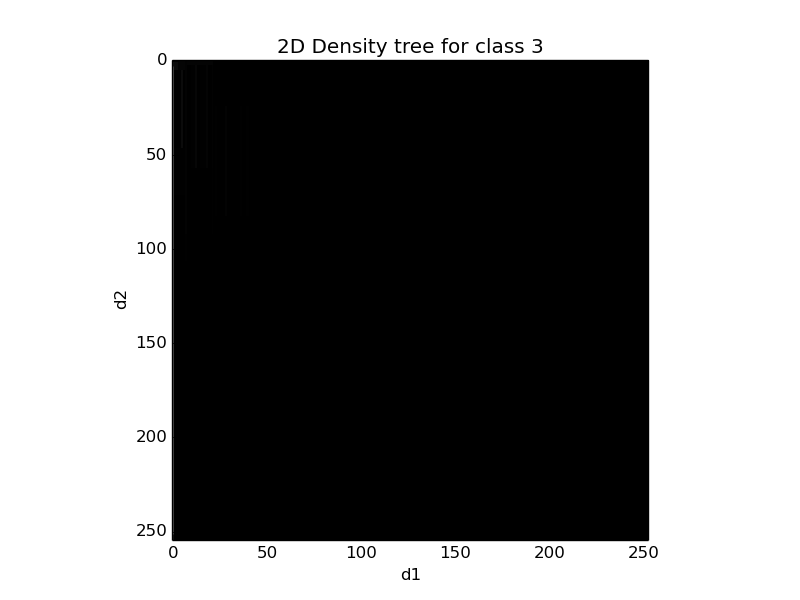
\includegraphics[width=\textwidth]{../naiveDT3.png}
                \caption{Class of handwritten threes}
        \end{subfigure}%
        \begin{subfigure}[b]{0.5\textwidth}
                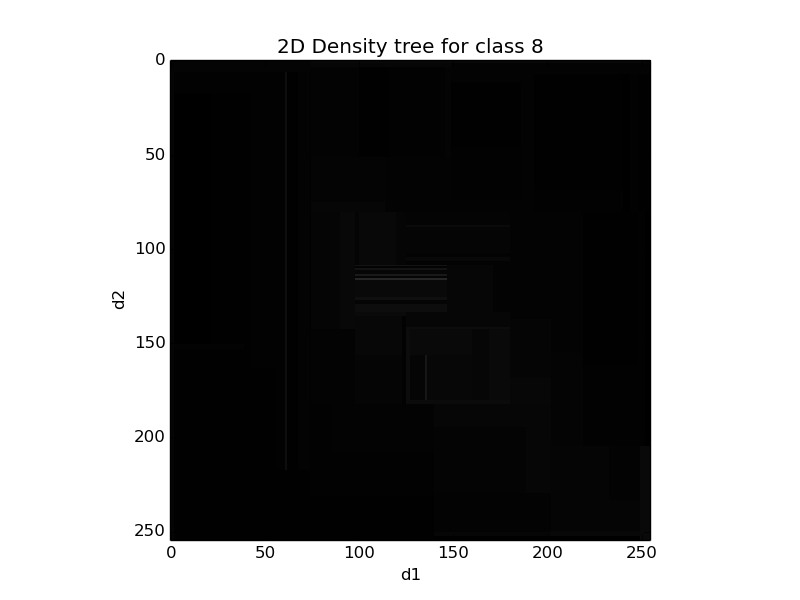
\includegraphics[width=\textwidth]{../naiveDT8.png}
                \caption{Class of handwritten eights}
        \end{subfigure}
        \caption{Adaptive bins for the density trees with naive splitting criterion}
        \label{img4}
\end{figure}


\FloatBarrier

\begin{lstlisting}[language=Python]
def DT_Classifier_2classes(testx, prior1, prior2, DT1, DT2, c = [3,8]):
    n = testx.shape[0]
    
    prediction = np.zeros(n, dtype = np.int8)
    
    for i in range(0,n):
        x = testx[i,:]
            
        # p(y = 3| x)
        # find right bin in DT:
        likelihood1 = 0
        for node in DT1:
            if point_in_region(x, node.region):
                likelihood1 = node.p
                break 
            # end if
        # end for node
        p_y1_x = likelihood1*prior1
           
        # p(y = 8| x) 
        # find right bin in DT:
        likelihood2 = -1
        for node in DT2:
            if point_in_region(x, node.region):
                likelihood2 = node.p
                break 
            # end if
        # end for node        
        p_y2_x = likelihood2*prior2
           
        # argmax (p_y3_x, p_y8_x) 
        if p_y1_x>p_y2_x :
            prediction[i] = c[0]
        else:
            prediction[i] = c[1]
        # end if        
           
    # end for i
    
    return prediction
# end DT_Classifier
\end{lstlisting}


\subsection{Generate threes}
For generation of new digits from the given likelihood function we implemented the following algorithm:
\begin{itemize}
\item use the whole dimensional training set to train the density tree for the digit $3$
\item start from the root node of the DT
\item with the selected probability $q$ go left in the tree and with probability $1-q$ go right; set $q=q*N_left/N$
\item repeat selection of the next node until a leaf node is reached
\item in the reached leaf node sample the points uniformly for each dimension
\end{itemize}

Here is the code to the described algorithm:
The traversal of the tree is done recursive with function $DT\_traverse$.

\begin{lstlisting}[language=Python]
## Generate Number from the given pdf
# samply in each of d dimensions independently
def generate_number(DT, trainingx,trainingy, c):
    # find  in training set all members of the class c
    xc = trainingx[trainingy==c, :]        
    N = xc.shape[0]
    d = xc.shape[1]

    ## Root node
    region = np.zeros((d,2), dtype = np.float32)
    for j in range(0,d):
        region[j,0] = np.min(xc[:,j])
        region[j,1] = np.max(xc[:,j])
    # end j   
        
    rootnode = DTnode(xc, 1/volume(region), region)
    pmin = 1.
    pmax = 0.
    for node in DT:
        if node.p>pmax:
            pmax = node.p
        if node.p<pmin:
            pmin = node.p
    #end for    
        
    # number of all points, probability to go left, root node, depth
    selectednode = DT_traverse(N, pmin, pmax, 0.5, rootnode, 0) 
    # in the leaf node sample uniformly in each direction
    newnumber = np.zeros(d, dtype = np.int32) 
    for j in range(0,d):
        a = selectednode.region[j,0]
        b = selectednode.region[j,1]
        
        alpha = random.random()
        # transforme random number in [0,1) in random number in [a,b)
        newnumber[j] = np.floor(a + alpha*(b-a))
    # for j    
    return newnumber
# def generate_number(pdf)    
\end{lstlisting}

\begin{lstlisting}[language=Python]
# traverse the density tree: go left with probability q and right with 
# probability 1-q, generate a uniform distributed number in range [qmin, qmax)
def DT_traverse(N, qmin, qmax, q, parentnode, depth):

    # if termination condition is satisfied (same as in construction of DT)
    pointsdensity = parentnode.points.shape[0]/float(N)
    if parentnode.p>=0.0001 or pointsdensity<0.001: 
        return parentnode
    else:
        # split value : split on the middle of the interval
    
        splitval, splitdim = splitnaive(parentnode, depth)

        # split poins of the node according to the new regions
        pointsL, pointsR = splitpoints(parentnode.points,parentnode.region,\
        					splitval, splitdim)
        
        x = random.uniform(qmin,qmax)        
        if x<=q:
            # split region
            region = np.copy(parentnode.region)
            region[splitdim,:] = [region[splitdim,0], splitval]            
            points = pointsL
        else:
            # split region
            region = np.copy(parentnode.region)       
            region[splitdim,:] = [splitval, region[splitdim,1] ]
            points = pointsR
        # else if
        
        # calculate new p
        q *= points.shape[0]/float(N)
        
        # go deeper
        node = DTnode(points, points.shape[0]/float(N)/volume(region), region)
        return DT_traverse(N, qmin, qmax, q, node, depth+1)
    # end if    
# end DT_traverse()
\end{lstlisting}        
 
 
Unfortunately, as you can seen on the next images this algorithm didn't provide good generation results.
\begin{figure}[ht]
        \centering
        \begin{subfigure}[b]{0.5\textwidth}
                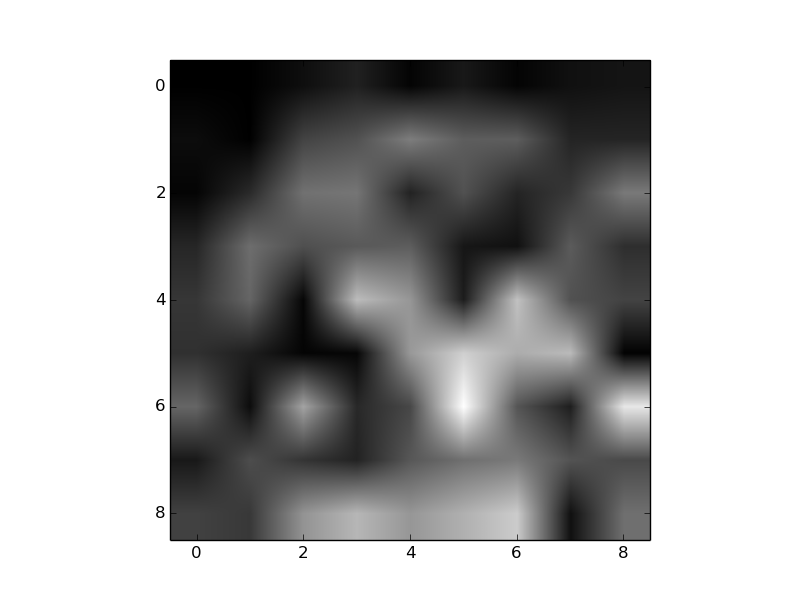
\includegraphics[width=\textwidth]{../new3DTn_1.png}
        \end{subfigure}%
        \begin{subfigure}[b]{0.5\textwidth}
                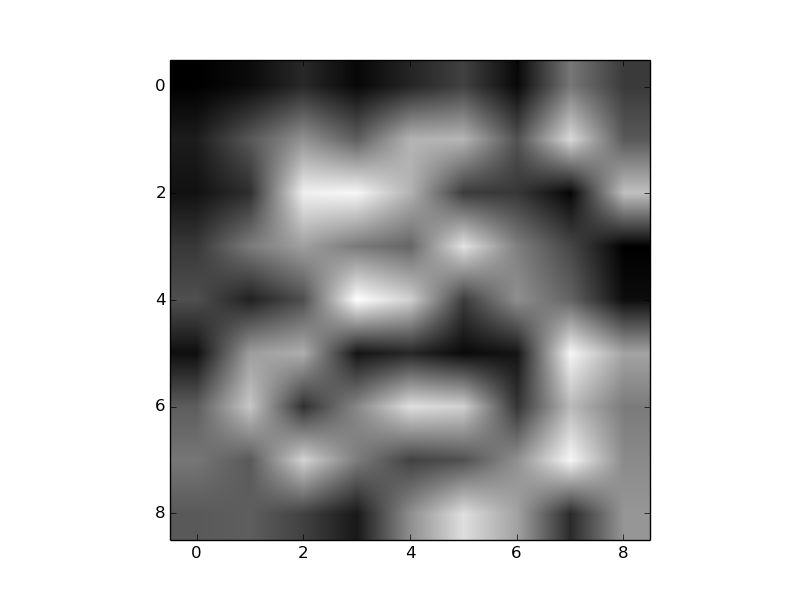
\includegraphics[width=\textwidth]{../new3DTn_2.png}
        \end{subfigure}
        \begin{subfigure}[b]{0.5\textwidth}
                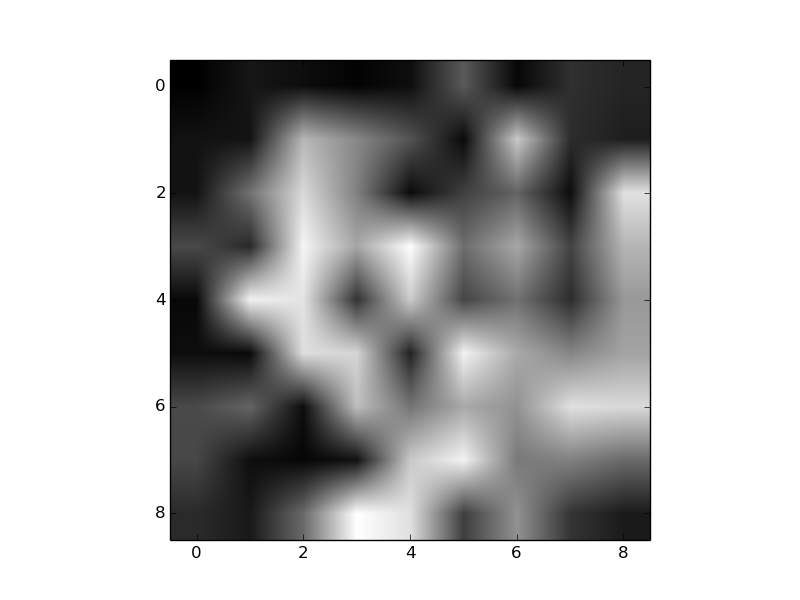
\includegraphics[width=\textwidth]{../new3DTn_3.png}
        \end{subfigure}        
        \caption{Generated threes}
\end{figure}

\FloatBarrier
All function from this section can be found in the $densityTree.py$ file in attachment.


\section{Combination of the density tree and Naive Bayes}
Unfortunately we didn't finished the implementation of the tasks in this section. That is why we provide only learning step for the method, that combines density tree with the naive Bayes method.

\begin{lstlisting}[language=Python]
    print    
    print "Classification"
    print    
    
   # train 1D-histogramms for each feature and class      
    
    tstart = time.time() 
    L, dx = chooseBinSize(images_train_38) # number of bins, bins size
    
    # pdf d x L matrices                  
    prior3, pdf3 = naiveBayes_train_single_class(images_train_38, \
                                                  labels_train_38, 3, dx, L)    
    prior8, pdf8 = naiveBayes_train_single_class(images_train_38, \
                                                  labels_train_38, 8, dx, L)    
    # compute the cdf of each histogramm
    cdf3 = np.zeros(pdf3.shape, dtype = np.float32)   
    cdf8 = np.zeros(pdf8.shape, dtype = np.float32)   
    for j in range(0, d):
        cdf3[j,:] = np.cumsum(pdf3[j,:])
        cdf8[j,:] = np.cumsum(pdf8[j,:])
    # end for                                               

    tstop = time.time()
    print "Learning 1D histograms and computing cdf's took {} sec".\
                                                        format(tstop-tstart)
    
    # map data to copula using rank order transformation
    u = np.zeros(images_train_38.shape, dtype = np.float32)
    for j in range(0,d):
        ind = np.sort(images_train_38[:,j])
        u[:,j] = ind[:]/float(n+1)
    # end for j    
    
    # train a DT on u
    tstart = time.time() 
    
    prior3, DT3 = DT_learning(u, labels_train_38, 3, 'naive') 
    prior8, DT8 = DT_learning(u, labels_train_38, 8, 'naive') 
    
    tstop = time.time()
    print "Learning DTs took {} sec". format(tstop-tstart)    
    
    print    
    print "Classification"
    print    
    
    ntest = images_test.shape[0]
    prediction = np.zeros(ntest, dtype = np.int8)
        
    for i in range(0,n):
        x = images_test[i,:]
        // u_j = F_j(x_j) 
        u3 = np.zeros(d, dtype = np.float32)        
        u8 = np.zeros(d, dtype = np.float32)                
        
        # compute density according to naive Bayes method
        naiveBayesDensity3 = 1.
        naiveBayesDensity8 = 1.        
        for j in range(0, d):
            l= np.floor(x[j]/dx[j])+1 # bin number
            if l>L-1:
                l=L-1
            naiveBayesDensity3 *= pdf3[j,l]            
            naiveBayesDensity8 *= pdf8[j,l]                      
            
            u3[j]= cdf3[j,l]
            u8[j]= cdf8[j,l]
        # end for j
        
        copulaDensity3 = 0
        for node in DT3:
            if point_in_region(u3, node.region):
                copulaDensity3 = node.p
                break 
            # end if
        # end for node
                
        copulaDensity8 = 0
        for node in DT8:
            if point_in_region(u8, node.region):
                copulaDensity8 = node.p
                break 
            # end if
        # end for node
                
        p_y3_x = naiveBayesDensity3*copulaDensity3*prior3
        p_y8_x = naiveBayesDensity8*copulaDensity8*prior8
        
        # argmax (p_y3_x, p_y8_x) 
        #print p_y3_x
        if p_y3_x>p_y8_x :
            prediction[i] = 3
        else:
            prediction[i] = 8
        # end if        
    # end for i    
\end{lstlisting}    


\section{Complete code}
\subsection{Naive Bayes method}
\lstinputlisting[language=Python]{../naiveBayes.py}
\subsection{Density tree method}
\lstinputlisting[language=Python]{../densityTree.py}
\subsection{Main function and Task 3}
\lstinputlisting[language=Python]{../ex04.py}

\end{document}
%------------------------------------------------------------------------------%                                    
